\usetikzlibrary{arrows}
\definecolor{zzttqq}{rgb}{0.6,0.2,0}
\definecolor{xdxdff}{rgb}{0.49019607843137253,0.49019607843137253,1}
\definecolor{uuuuuu}{rgb}{0.26666666666666666,0.26666666666666666,0.26666666666666666}
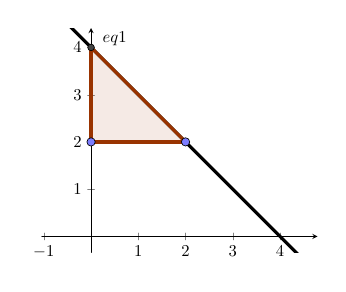
\begin{tikzpicture}[line cap=round,line join=round,>=triangle 45,x=1cm,y=1cm,scale=.6]
    \begin{axis}[
            x=1cm,y=1cm,
            axis lines=middle,
            xmin=-1.0430999574123194,
            xmax=4.793645986891604,
            ymin=-0.3419648743673125,
            ymax=4.411066384011339,
            xtick={-1,0,...,4},
            ytick={0,1,...,4},]
        \clip(-1.0430999574123194,-0.3419648743673125) rectangle (4.793645986891604,4.411066384011339);
        \fill[line width=2pt,color=zzttqq,fill=zzttqq,fill opacity=0.10000000149011612] (0,4) -- (0,2) -- (2,2) -- cycle;
        \draw [line width=2pt,domain=-1.0430999574123194:4.793645986891604] plot(\x,{(--4-1*\x)/1});
        \draw [line width=2pt,color=zzttqq] (0,4)-- (0,2);
        \draw [line width=2pt,color=zzttqq] (0,2)-- (2,2);
        \draw [line width=2pt,color=zzttqq] (2,2)-- (0,4);
        \begin{scriptsize}
            \draw[color=black] (0.5,4.184310865488937) node {$eq1$};
            \draw [fill=uuuuuu] (0,4) circle (2pt);
            \draw [fill=xdxdff] (0,2) circle (2.5pt);
            \draw [fill=xdxdff] (2,2) circle (2.5pt);
        \end{scriptsize}
    \end{axis}
\end{tikzpicture}